\chapter{Dataset}

The success of any deep learning-based classification system heavily depends on the quality, diversity, and balance of the dataset used. In this research, we have developed a comprehensive mango leaf image dataset by merging two well-known public sources. The dataset represents a wide range of visual symptoms across eight different classes—seven disease categories and one healthy category. The collected data includes variations in lighting, background, camera angles, and disease stages, which helps to generalise the models to real-world conditions.

\subsection{Data Collection}

To develop a robust and generalizable model for mango leaf disease classification, we have utilized a high-quality datasets obtained from the Mendeley Data repository. This datasets collectively offer a diverse and balanced collection of mango leaf images representing both healthy and diseased categories. The images were captured under natural orchard conditions from multiple regions in Bangladesh, ensuring variability in lighting, angles, and background. This variation helps improve the model’s ability to generalize to unseen real-world scenarios.
\\
The dataset comprises \textbf{4,000 mango leaf images} captured in natural orchard conditions across four different locations in Bangladesh\cite{mangoleafbd}:

\begin{itemize}
    \item Sher-e-Bangla Agricultural University orchard
    \item Jahangirnagar University orchard
    \item Udaypur village mango orchard
    \item Itakhola village mango orchard
\end{itemize}

\textbf{Specifications:}
\begin{itemize}
    \item \textbf{Image Size:} 240 $\times$ 320 pixels
    \item \textbf{Format:} JPG
    \item \textbf{Classes:} 8 (7 diseased, 1 healthy)
    \item \textbf{Images per Class:} 500
    \item \textbf{Data Augmentation:} Around 2,200 images via rotation, zooming, and flipping
    \item \textbf{Acquisition Device:} Mobile phone cameras
\end{itemize}


\subsection{Data Statistics and Distribution}

After merging the two datasets, we ensured an equal number of samples across each class. Each of the eight classes now contains \textbf{1,300 images}, resulting in a final dataset of \textbf{10,400 images}.

\begin{table}[H]
\centering
\caption{Number of Images per Class}
\begin{tabular}{lccc}
\toprule
\textbf{Class} & \textbf{Dataset} \\
\midrule
Anthracnose       & 500  \\
Bacterial Canker  & 500  \\
Cutting Weevil    & 500  \\
Die Back          & 500 \\
Gall Midge        & 500 \\
Powdery Mildew    & 500 \\
Sooty Mould       & 500 \\
Healthy           & 500 \\
\midrule
\textbf{Total}    & \textbf{4000} \\
\bottomrule
\end{tabular}
\end{table}

\begin{figure}[H]
\centering
\caption{Image Count per Class}
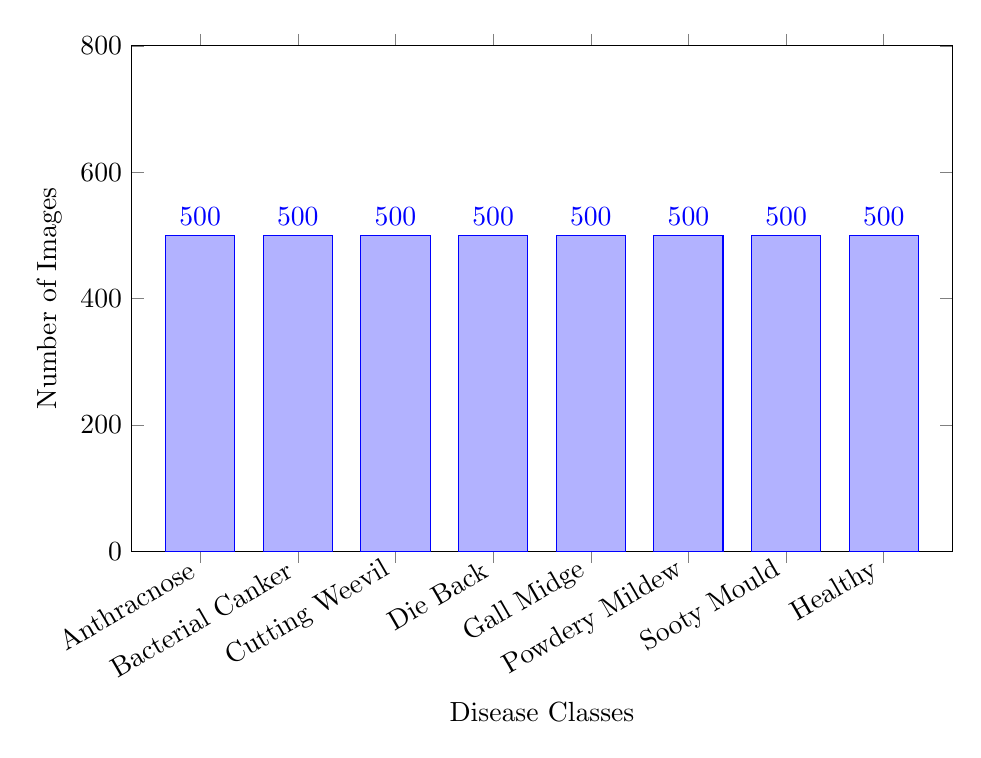
\begin{tikzpicture}
\begin{axis}[
    width=12cm,
    height=8cm,
    ybar,
    bar width=25pt,
    xlabel={Disease Classes},
    ylabel={Number of Images},
    symbolic x coords={Anthracnose,Bacterial Canker,Cutting Weevil,Die Back,Gall Midge,Powdery Mildew,Sooty Mould,Healthy},
    xtick=data,
    nodes near coords,
    enlarge x limits=0.1,
    xticklabel style={rotate=30, anchor=east},
    ymin=0, ymax= 800,
    ylabel near ticks,
    xlabel near ticks
]
\addplot coordinates {
    (Anthracnose,500)
    (Bacterial Canker,500)
    (Cutting Weevil,500)
    (Die Back,500)
    (Gall Midge,500)
    (Powdery Mildew,500)
    (Sooty Mould,500)
    (Healthy,500)
};
\end{axis}
\end{tikzpicture}
\end{figure}

\subsection{Disease Classes and Their Visual Features}

Each class in the dataset represents a specific mango leaf condition. Understanding the visual characteristics of each disease is important for both human inspection and model interpretability.

\begin{table}[H]
\centering
\caption{Visual Characteristics of Each Class}
\label{tab:disease-characteristics}
\renewcommand{\arraystretch}{1.5}
\begin{adjustbox}{width=\textwidth}
\begin{tabular}{@{}p{3.5cm}p{12cm}@{}}
\toprule
\textbf{Disease Class} & \textbf{Key Visual Characteristics} \\
\midrule
\textbf{Anthracnose} & Small, dark brown to black lesions with irregular shapes. Commonly starts at the leaf tip and may coalesce to form large necrotic areas. Lesions often have a concentric ring pattern and may lead to leaf curling or drying. \\

\textbf{Bacterial Canker} & Water-soaked lesions that enlarge and turn dark brown or black. Lesions are often angular and surrounded by yellow halos. Severe cases show cracking along veins and deformation of the leaf surface. \\

\textbf{Cutting Weevil} & Leaves show notched, chewed, or semi-circular cuts along the margins, caused by adult weevils feeding. Damage appears as clean cuts and may affect multiple edges of a single leaf. \\

\textbf{Die Back} & Yellowing and browning begins at the tip and progresses downward toward the base. May cause full leaf drying and extend into twigs. Often associated with poor plant vigor or fungal infection. \\

\textbf{Gall Midge} & Distinct swollen blisters, wart-like growths, or raised galls appear on leaf surfaces, particularly near veins. Caused by insect larvae feeding inside the tissue. \\

\textbf{Powdery Mildew} & A whitish or gray powder-like fungal coating appears on both surfaces, but mainly on the upper side. Advanced stages cover large areas and may distort leaves. \\

\textbf{Sooty Mould} & A black, soot-like fungal layer covers the leaf surface. Although the mold itself does not infect the plant, it blocks sunlight and photosynthesis. Often linked to honeydew secretions from insects. \\

\textbf{Healthy} & Uniform bright green color, smooth texture, no visible signs of necrosis, deformation, or discoloration. Veins and edges are clearly defined and free of lesions or foreign growth. \\
\bottomrule
\end{tabular}
\end{adjustbox}
\end{table}

\begin{figure}[h!]
    \centering
    \includegraphics[width=1.0\textwidth]{Figure/leaf.pdf}
    \caption{Representative Images of Each Class}
    \label{fig:pdf_example}
\end{figure}



These images and visual descriptions help in understanding the symptom patterns for each disease and serve as a visual reference for model training and evaluation.
